\documentclass[11pt,a4paper]{article}
\usepackage[utf8]{inputenc}
\usepackage[T1]{fontenc}
%\usepackage{gentium}
\usepackage{mathptmx} % Use Times Font

\usepackage{graphicx} % Required for including pictures
\usepackage{hyperref} % Format links for pdf
\usepackage{biblatex}
\addbibresource{references.bib}
\usepackage{booktabs} % Used so that tables generated by pandas
                      % to_latex() work correctly

\frenchspacing % No double spacing between sentences
\usepackage[margin=1in]{geometry}

\usepackage[all]{nowidow} % Tries to remove widows
\usepackage[protrusion=true,expansion=true]{microtype} % Improves typography, load after fontpackage is selected

\usepackage{lipsum} % Used for inserting dummy 'Lorem ipsum' text into the template

\title{My datascience project title}
\author{PUT YOUR EXAM NUMBER(S) HERE}

\begin{document}

\maketitle

%% INSTRUCTIONS:
%%
%% 1. Create your own copy of this Overleaf project. You can either edit your report
%% using:
%%
%%    a. Overleaf professional, a collaborative LaTeX editor. You can click
%%       "Copy Project" from the Overleaf menu to create a version where you have
%%       read and write permissions. See the following for documentation:
%%       https://www.overleaf.com/edu/edinburgh and
%%       https://uoe.sharepoint.com/:f:/r/sites/digitalskillsandtraining/Shared%20Documents/LaTeX/LaTeX%20for%20Beginners%20using%20Overleaf?csf=1&web=1&e=cPqTI3
%%
%%    b. A LaTeX editor on your PC. For this option, you can download the source
%%       of this project as a zip (via the Overleaf menu).
%% 
%% 2. Please rename this file fds-project-option-1.tex, 
%% fds-project-option-2.tex, or fds-project-option-3.tex, depending on
%% which project option you are doing. When you submit, please submit
%% the PDF file with the corresponding name.
%% 
%% 3. Please keep the section and paragraph headings as they
%%    are. You should delete all the text within the headings, e.g.
%%    the text that says "What is the area of this data science
%%    study, and why is it interesting to investigate" and the
%%    bullet points. Keeping the headings makes the report a lot
%%    easier for the markers to read, and making things easy for
%%    markers is always beneficial.
%%
%% 4. The word limit for the Overview section is mandatory. For the
%% other sections word limits are suggested.
%%
%% 5. The page limits must be strictly adhered to, and depend on if
%% you are working individually, in pairs or in threes:
%%
%%   - Individual: 6 pages 
%%   - Pairs: 8 pages 
%%   - Threes: 10 pages 
%%

\section{Overview}
% 250 words maximum

\section{Introduction}
% Suggested 400 words

\paragraph{Context and motivation}

What is the area of this data science study, and why is it interesting
to investigate?

\paragraph{Previous work}

Brief description of any previous work in this area (e.g., in the
media, or scientific literature or blogs).

E.g. Recent surveys show that most students prefer final projects to
final exams \cite{Space2021}.

\paragraph{Objectives}

What questions are you setting out to answer?

\section{Data}
% Suggested 300 words

\paragraph{Data provenance} Who created the dataset(s)?  How you have
obtained it (e.g., file or web scraping), and do the T\&Cs allow you
to use obtain the data for the project?

\paragraph{Data description} Description of the data, e.g. variables
in each table, number of records.

\paragraph{Data processing} How you have processed the dataset, e.g.,
cleaning, removing missing values, joining tables.

\section{Exploration and  analysis}
% Suggested 500 words for individual report; proportionately longer
% for group projects).

% 't' means "try to position at the top of the page"
\begin{figure}[t]
  \centering
  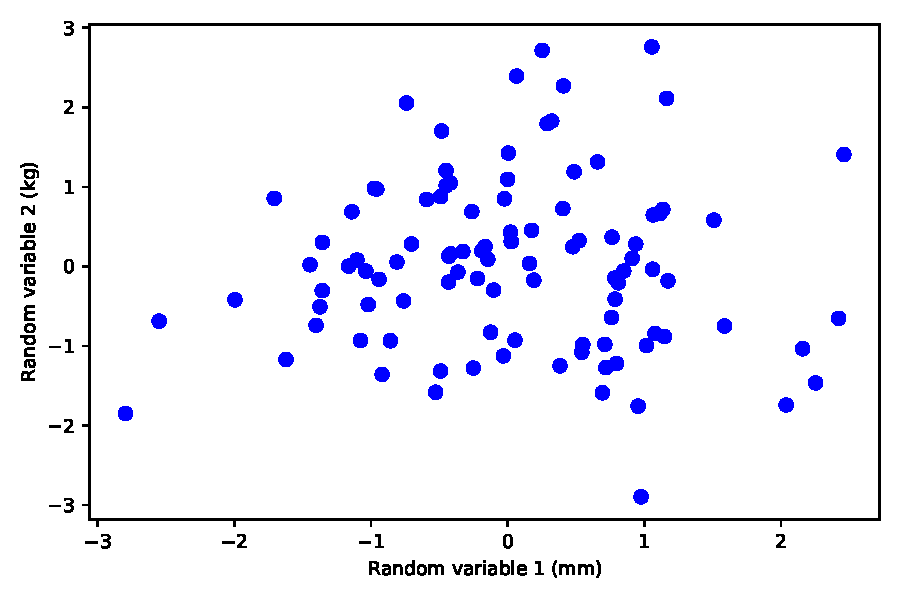
\includegraphics{example1}
  \caption{Demonstration figure. This caption explains more about the
    figure. Note that the font size of the labels in the plot is 9pt,
    which is obtained by the settings as shown in the Jupyter
    notebook.}
  \label{fds-project-template:fig:example1}
\end{figure}

% 'b' means "try to position at the bottom of the page"
\begin{table}[b]
  \centering
  \caption{Excerpt from Scottish Index of Multiple Deprivation, 2016 edition.
    \url{https://simd.scot}. You may put more information in the caption.}
  \label{tab:example1}
\begin{tabular}{lrrrrrrr}
\hline\hline
\textbf{Location}&\textbf{Employ-}&\textbf{Illness}&\textbf{Attain-}&\textbf{Drive}  &\textbf{Drive}    &\textbf{Crime}&\dots\\
                 &\textbf{ment}   &                &\textbf{ment}   &\textbf{Primary}&\textbf{Secondary}&              &\\
\hline
\textbf{Macduff}&$10$&$ 95$&$5.3$&$1.5$&$6.6$&$249$&\dots\tabularnewline
\textbf{Kemnay}&$ 3$&$ 40$&$5.3$&$2.4$&$2.4$&$168$&\dots\tabularnewline
\textbf{Hilton}&$ 0$&$ 10$&$6.3$&$2.2$&$3.0$&$144$&\dots\tabularnewline
\textbf{Ruchill}&$ 8$&$130$&$4.9$&$1.7$&$5.6$&$318$&\dots\tabularnewline
\textbf{Belmont}&$ 2$&$ 50$&$6.1$&$3.1$&$3.2$&$129$&\dots\tabularnewline
\dots&\dots&\dots&\dots&\dots&\dots&\dots&\dots\tabularnewline
\hline
\end{tabular}
\end{table}

A data science analysis of the paper, including: 
\begin{itemize}
\item Visualisations (for example
  Figure~\ref{fds-project-template:fig:example1}) and tables (for
  example Table~\ref{tab:example1}). Please make sure that all figures
  and tables are referred to in the text, as demonstrated in this
  bullet point.
\item Interpretation of the results 
\item Description of how you have applied one ore more of the
  statistical and ML methods learned in the FDS to the data
\item Interpretation of the findings 
\end{itemize}

You can use equations like this:
\begin{equation}
  \label{fds-project-template:eq:1}
  \overline{x} = \sum_{i=1}^n x_i
\end{equation}
or maths inline: $E=mc^2$. However, you do not need to reexplain techniques that you have learned in the course -- assume the reader understands linear regression, logistic regression K-nearest neighbours etc.  Remember to explain any symbols use, e.g.~``$n$ is the number of data points and $x_i$ is the value of the $i$th data point.''.

\section{Discussion and conclusions}
% Suggested 400 words.

\paragraph{Summary of findings}

\paragraph{Evaluation of own work: strengths and limitations}

\paragraph{Comparison with any other related work}
E.g. ``Anscombe has also demonstrated that many patterns of data can
have the same correlation coefficient'' \cite{anscombe1973graphs}.

Wikipedia can also be cited but it is better if you find the original
reference it for a particular claim in the list of references on the
Wikipedia page, read it, and cite it.

The golden rule is always to cite information that has come from other
sources, to avoid plagiarism \cite{wiki:plagarism}.

\paragraph{Improvements and extensions}


\printbibliography
\end{document}

% LocalWords:  lrrrrrrr ment Macduff Kemnay Ruchill FDS mc th fds
% LocalWords:  Anscombe